\chapter{Oracle Aplication Express}

\section{Pengenalan Oracle APEX}
Oracle Aplication Express\cite{OracleApex}. Adalah sebuah wadah dan sarana untuk membuat aplikasi yang menggunakan database Oracle Itu sendiri, pada kelas Online pertama saya belajar banyak hal cara Menggunakan Aplikasi Oracle Apex online yang di dalam video sudah diberikan link diantaranya Request Workspace, Create Workspace, Membuat Spreadsheet Pertama.

\section{Tahapan Membuat Aplikasi Oracle Apex}
Pertama kita membuka website https://apex.oracle.com, disini kita akan mendapatkan akses untuk memasuki Oracle Apllication Express, siapkan email anda yang valid untuk membuat Workspace, kita akan langsung mempraktekan bagaimana tahapan pembuatan Aplikasi pada Oracle APEX :

\begin{enumerate}
\item[1]Klik Get Start For Free.

\begin{figure}[!htbp]
    \begin{center}
    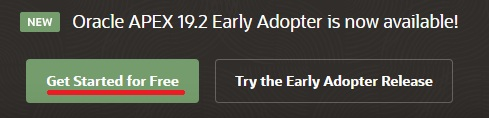
\includegraphics[scale=0.7]{figures/start.jpg}
    \caption{\textit{Get Start For Free.}}
    \end{center}   
    \end{figure}
    
\begin{figure}[!htbp]
\item[2]Klik Request a Free Worksace.

    \begin{center}
    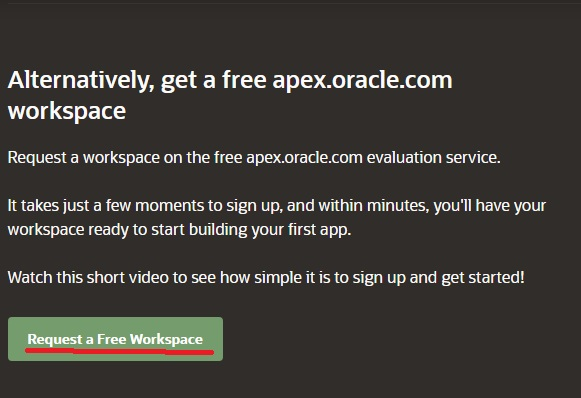
\includegraphics[scale=0.5]{figures/request_wspace.jpg}
    \caption{\textit{Request A Free Workspace.}}
    \end{center}

\item[3]Isikan data diri anda seperti nama,email,dan workspace.

    \begin{center}
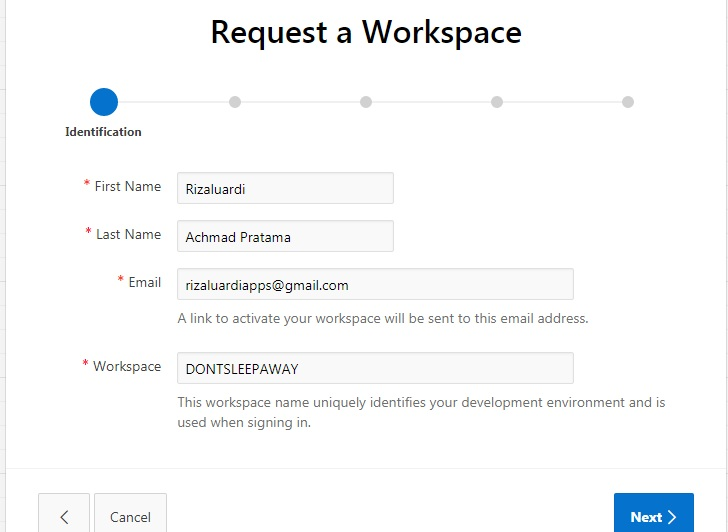
\includegraphics[scale=0.4]{figures/req1.jpg}
    \caption{\textit{Data Diri.}}
        \end{center}
        
\item[4]Centang apakah anda pernah melakukan hal tersebut lalu next.  

    \begin{center}
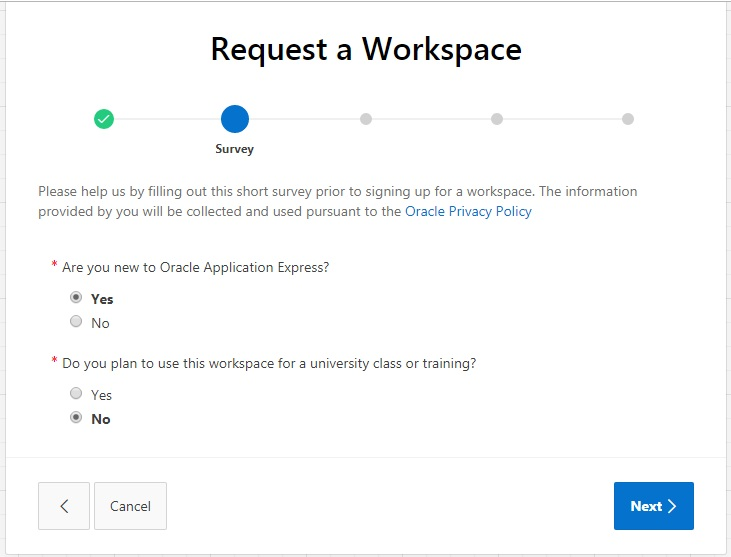
\includegraphics[scale=0.4]{figures/req2.jpg}
    \caption{\textit{Data Diri 2.}}
        \end{center}
        \end{figure}

\begin{figure}
\item[5]Isikan pada kolom tersebut bebas, mengapa anda ingin menggunakan layanan ini ?, lalu klik next.

    \begin{center}
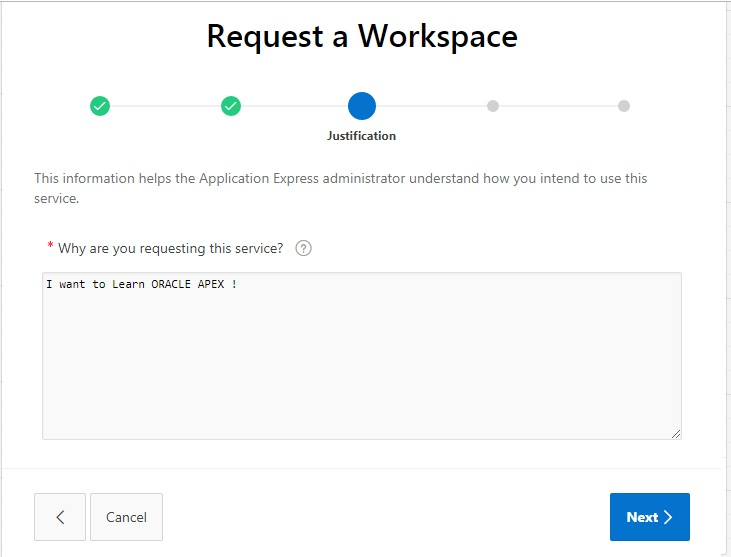
\includegraphics[scale=0.5]{figures/req3.jpg}
    \caption{\textit{Mengapa anda memakai oracle ?.}}
        \end{center}

\label{gambar}
\end{figure}

\begin{figure}
\item[6] Centang Accept, lalu klik next.

    \begin{center}
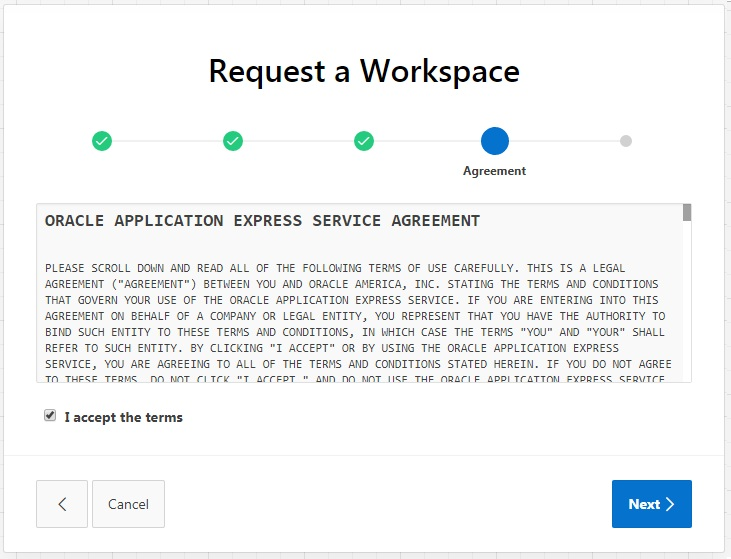
\includegraphics[scale=0.5]{figures/req4.jpg}
    \caption{\textit{Peringatan pengunaan.}}
        \end{center}

\label{gambar}
\end{figure}

\begin{figure}
\item[7] Tahapan terakhir untuk mengkonfirmasi apakah ini anda, lalu klik next.

    \begin{center}
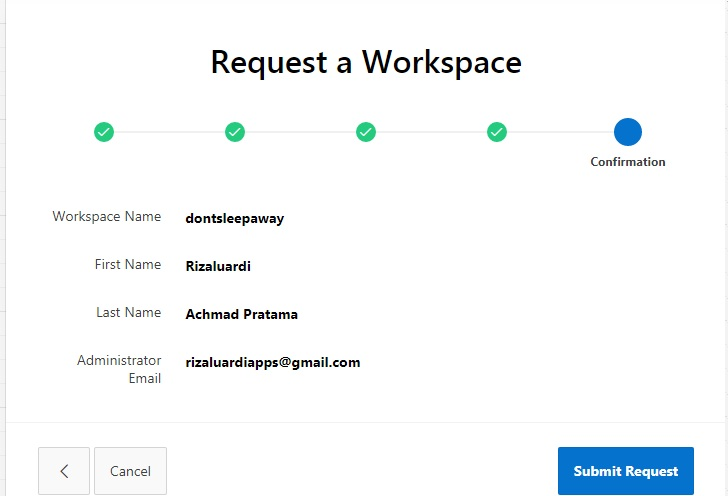
\includegraphics[scale=0.5]{figures/req5.jpg}
    \caption{\textit{Konfirmasi.}}
        \end{center}
\label{gambar}
\end{figure}

\begin{figure}
\item[8] Finish, lalu lihat email anda.

    \begin{center}
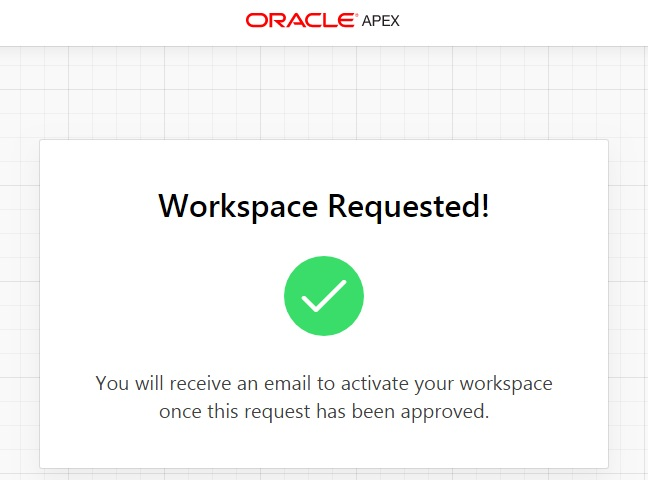
\includegraphics[scale=0.5]{figures/req6.jpg}
    \caption{\textit{Sukses Cek Email.}}
        \end{center}
\label{gambar}
\end{figure}

\begin{figure}
\item[9] Selamat Workspace anda telah di Acc lalu klik continue.

    \begin{center}
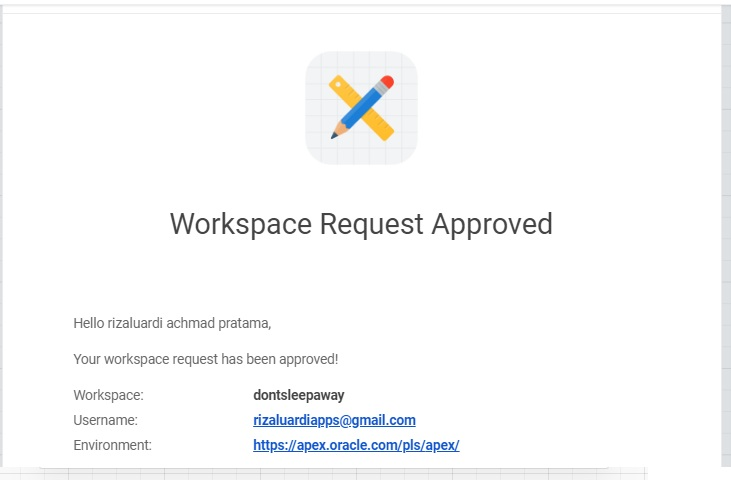
\includegraphics[scale=0.5]{figures/req7.jpg}
    \caption{\textit{Email Acc.}}
        \end{center}
\label{gambar}
\end{figure}

\begin{figure}
\item[10] Workspace kamu telah dibut lalu lanjutkan klik sign in.

    \begin{center}
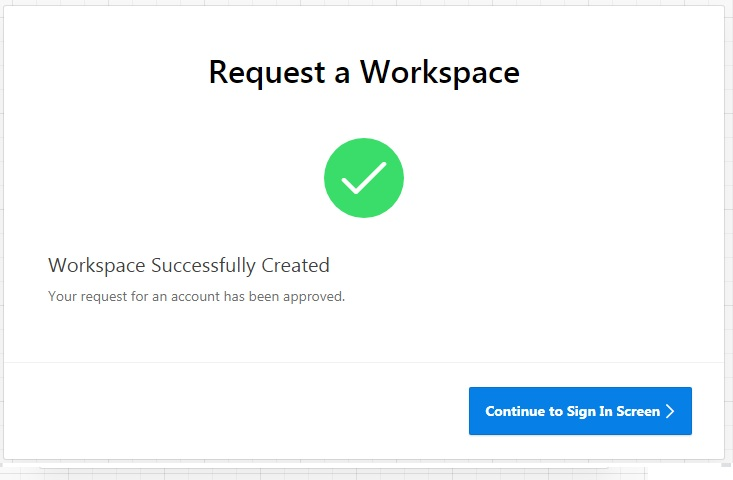
\includegraphics[scale=0.5]{figures/req8.jpg}
    \caption{\textit{Sukses Cek Email.}}
        \end{center}
\label{gambar}
\end{figure}

\begin{figure}
\item[11] Sign in akun anda yang baru saja di buat.

    \begin{center}
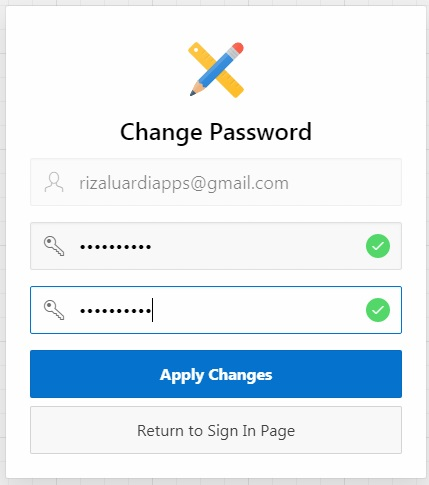
\includegraphics[scale=0.5]{figures/req9.jpg}
    \caption{\textit{Sign in oracle.}}
        \end{center}
\label{gambar}
\end{figure}

\begin{figure}
\item[12] Selamat, anda masuk Tampilan halaman awal aplikasi Oracle Express.

    \begin{center}
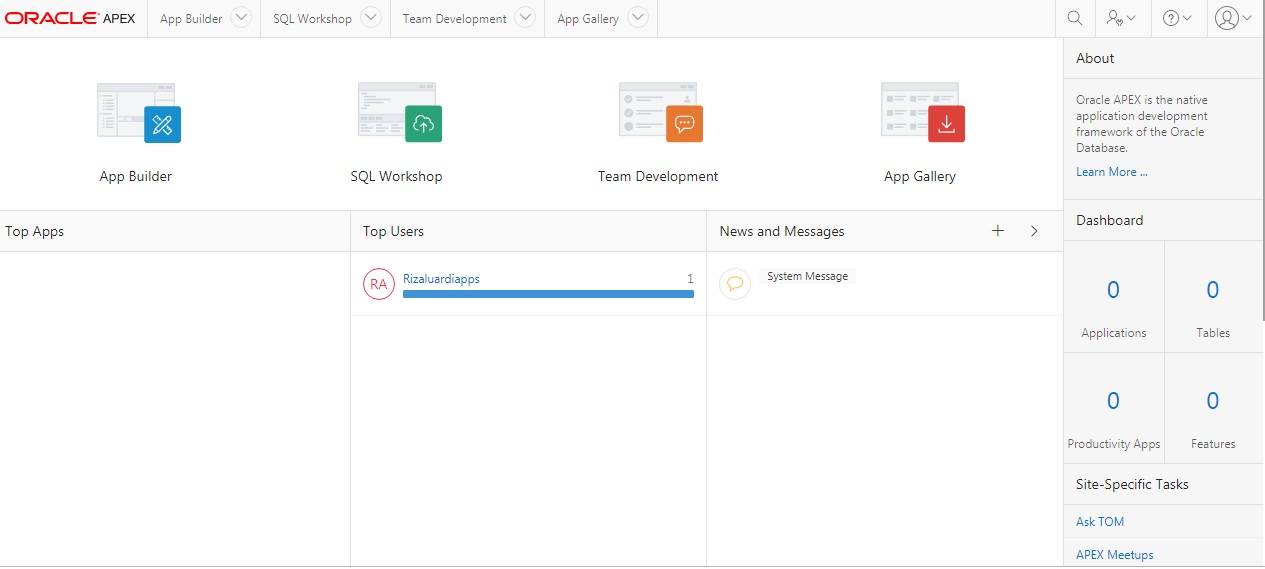
\includegraphics[scale=0.4]{figures/login1.jpg}
    \caption{\textit{Oracle Apex Home.}}
        \end{center}
\label{gambar}
\end{figure}

\begin{figure}
\item[13] Lalu buka App Builder klik Create New App.

    \begin{center}
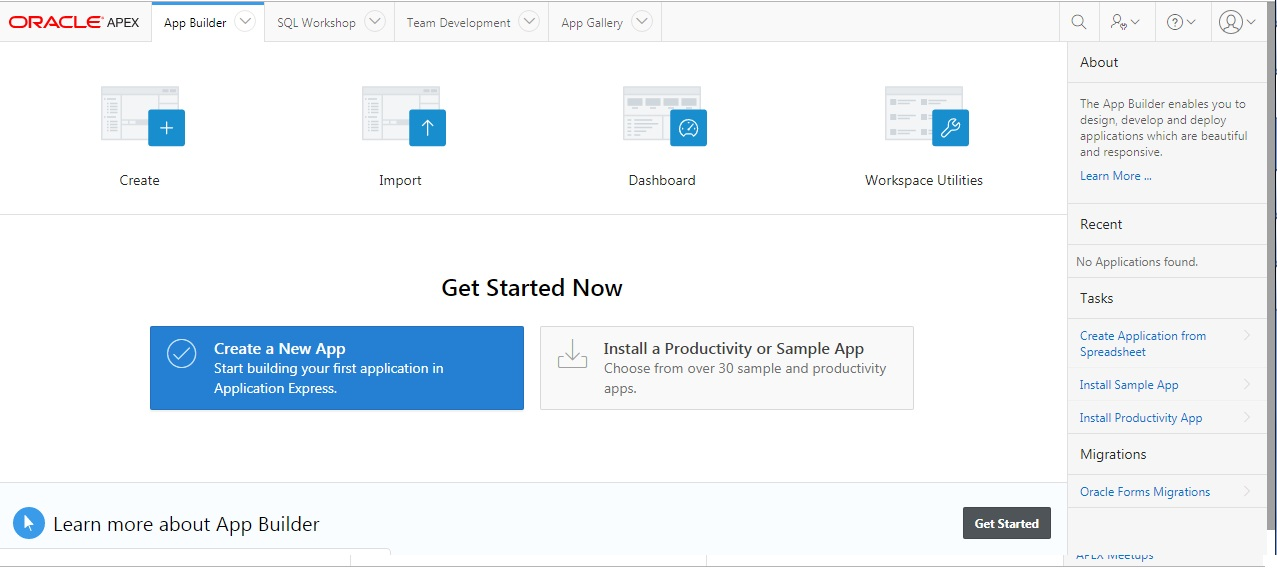
\includegraphics[scale=0.4]{figures/login2.jpg}
    \caption{\textit{Oracle Apex App Builder.}}
        \end{center}
\label{gambar}
\end{figure}

\begin{figure}
\item[14] Pilih Copy and Paste, pada select data CSV pilih Project and Tables lalu next.

    \begin{center}
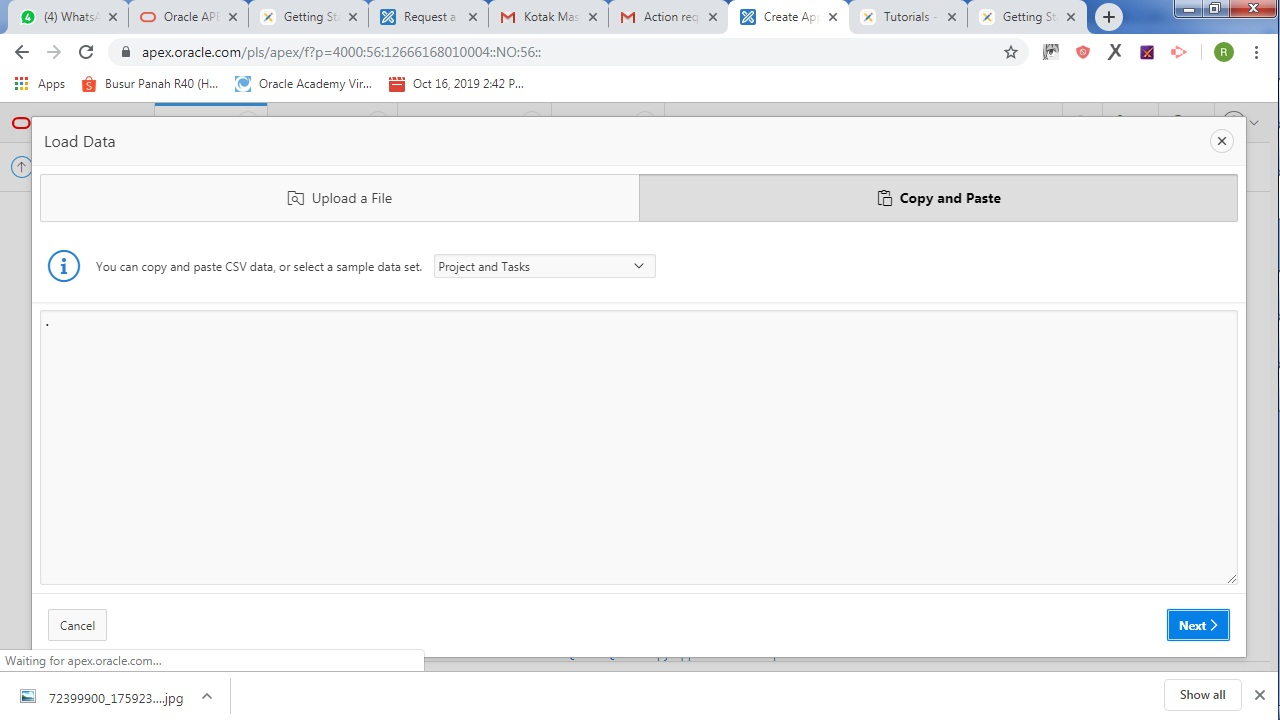
\includegraphics[scale=0.4]{figures/login3.jpg}
    \caption{\textit{Oracle Apex App Builder2.}}
        \end{center}
\label{gambar}
\end{figure}

\begin{figure}
\item[15] Setelah Sudah me-Load data, tampilan selanjutnya akan seperti berikut.

    \begin{center}
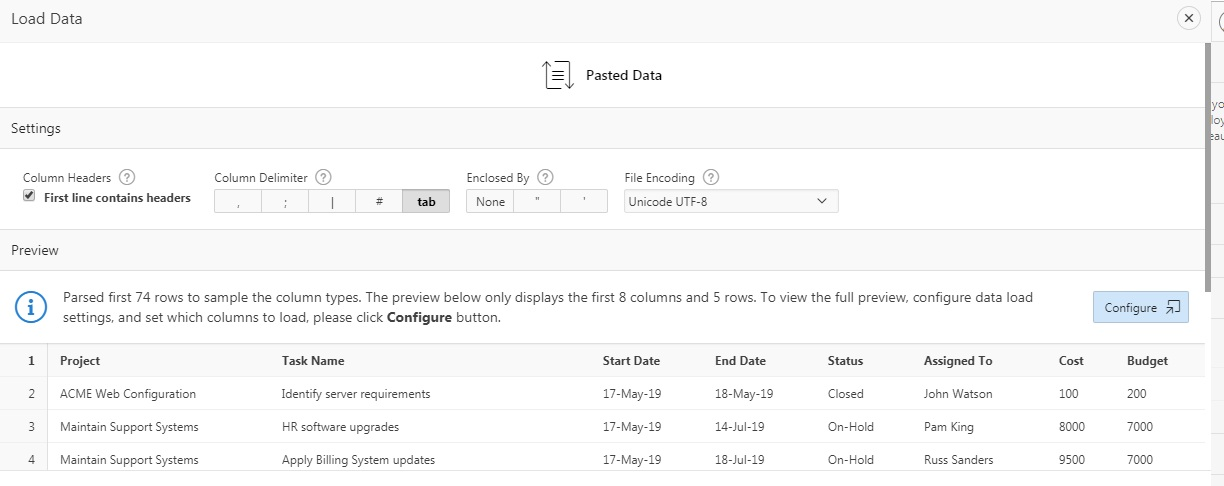
\includegraphics[scale=0.4]{figures/login4.jpg}
    \caption{\textit{Oracle Apex Load Data.}}
        \end{center}
\label{gambar}
\end{figure}

\begin{figure}
\item[16] Scroll ke bwah lalu setting Table Owner,Table Name,Error Table Name, dan Primary Keys, seperti gambar berikut.

    \begin{center}
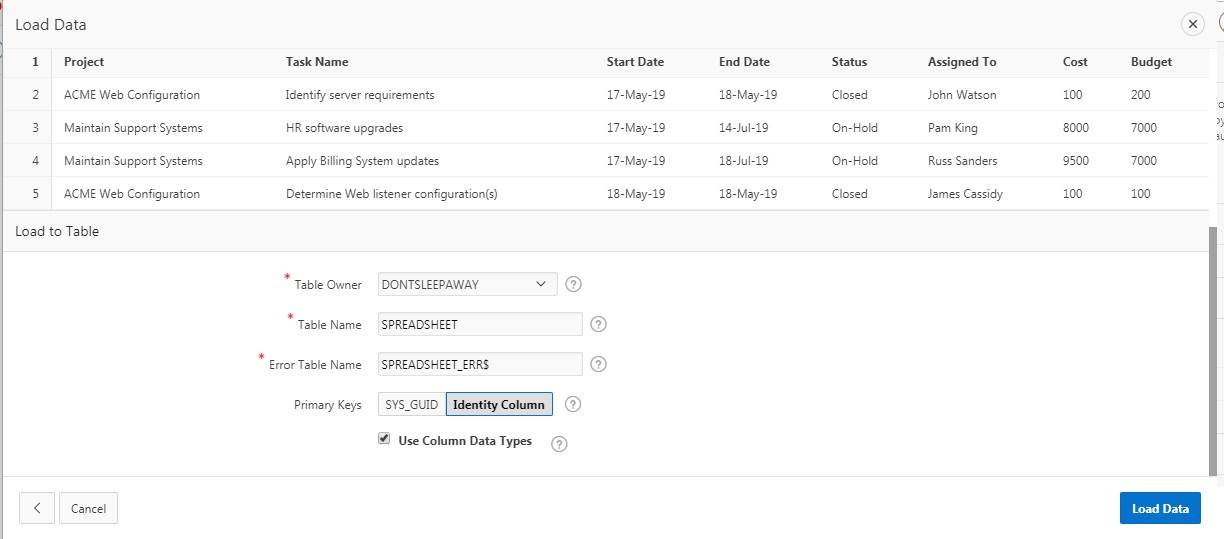
\includegraphics[scale=0.4]{figures/login5.jpg}
    \caption{\textit{Oracle Apex Load Data2.}}
        \end{center}
\label{gambar}
\end{figure}

\begin{figure}
\item[17] Load Data Sukses , klik Continue to Create Aplication Wizard.

    \begin{center}
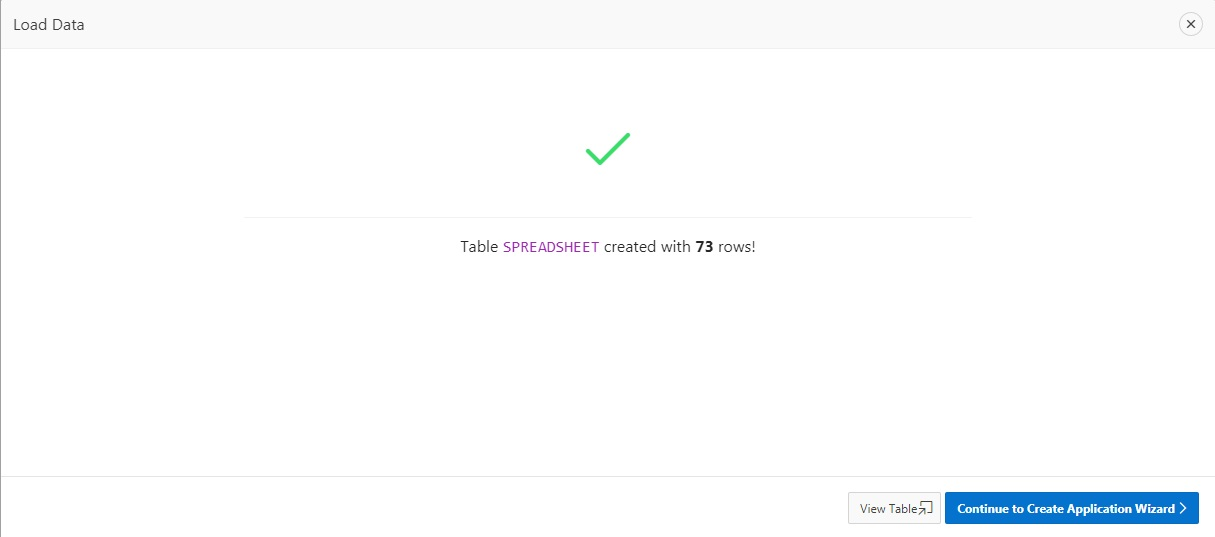
\includegraphics[scale=0.4]{figures/login6.jpg}
    \caption{\textit{Oracle Apex Load Data Success.}}
        \end{center}
\label{gambar}
\end{figure}

\begin{figure}
\item[18] Sekarang anda ada di tampilan Create an Aplication, ikuti langkah berikut, buat nama App from a Spreadsheet lalu pada Features klik Check All.

    \begin{center}
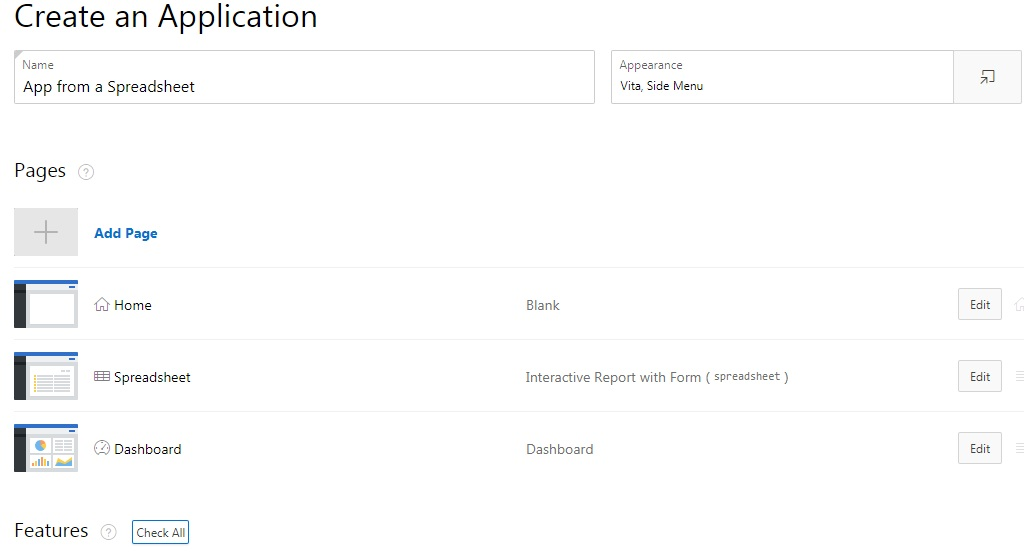
\includegraphics[scale=0.4]{figures/create1.jpg}
    \caption{\textit{Create an Aplication.}}
        \end{center}
\label{gambar}
\end{figure}


\begin{figure}
\item[19]Scroll ke bawah lalu klik Create Application .

    \begin{center}
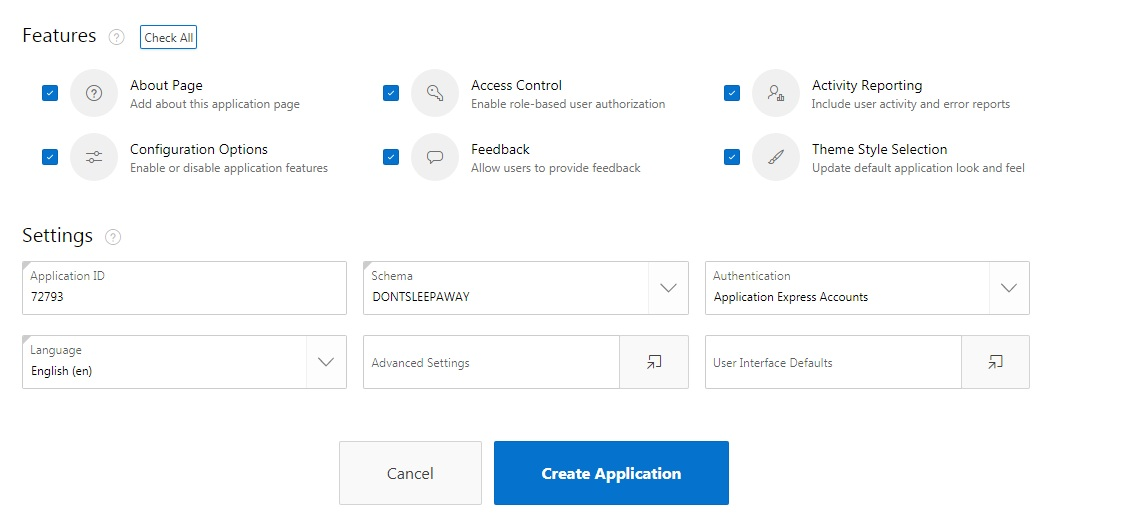
\includegraphics[scale=0.4]{figures/create2.jpg}
    \caption{\textit{Create an Application 2.}}
        \end{center}
\label{gambar}
\end{figure}

\begin{figure}
\item[20]Tunggu sebentar, data sedang dimuat .

    \begin{center}
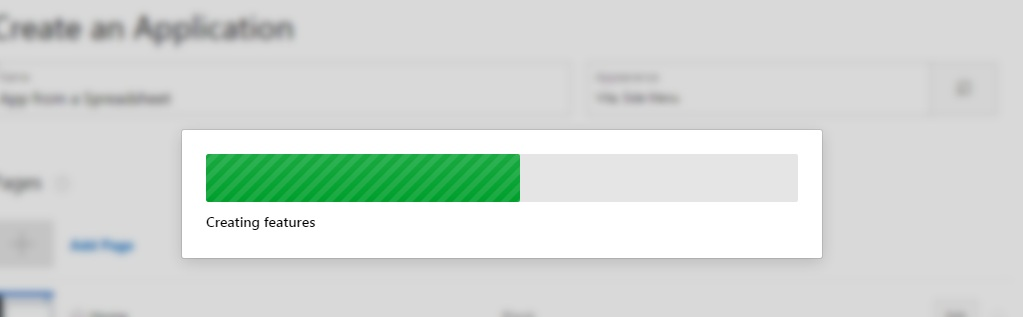
\includegraphics[scale=0.4]{figures/create3.jpg}
    \caption{\textit{Loading Data.}}
        \end{center}
\label{gambar}
\end{figure}

\begin{figure}
\item[21]Anda akan masuk ke halaman App Builder project Spreadsheet telah berhasil dibuat !, lalu klik Run application .

    \begin{center}
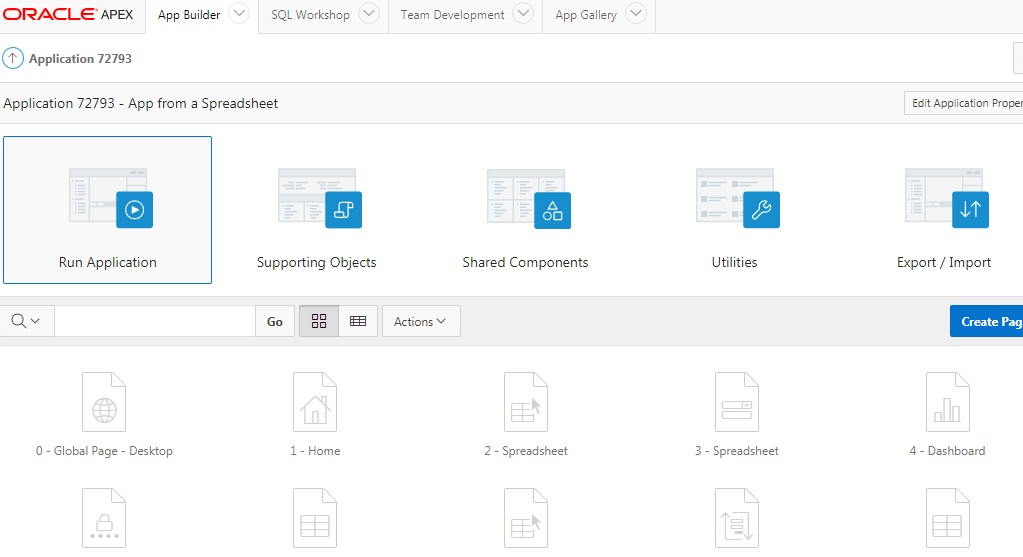
\includegraphics[scale=0.4]{figures/create4.jpg}
    \caption{\textit{App Builder Done!.}}
        \end{center}
\label{gambar}
\end{figure}

\begin{figure}
\item[22]Login ke Aplikasi anda menggunakan login Oracle APEX .

    \begin{center}
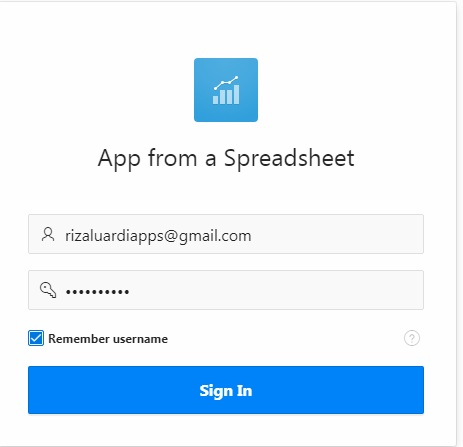
\includegraphics[scale=0.4]{figures/create5.jpg}
    \caption{\textit{Sign In Spreadsheet.}}
        \end{center}
\label{gambar}
\end{figure}

\begin{figure}
\item[23]Selamat Aplikasi telah berjalan ! .

    \begin{center}
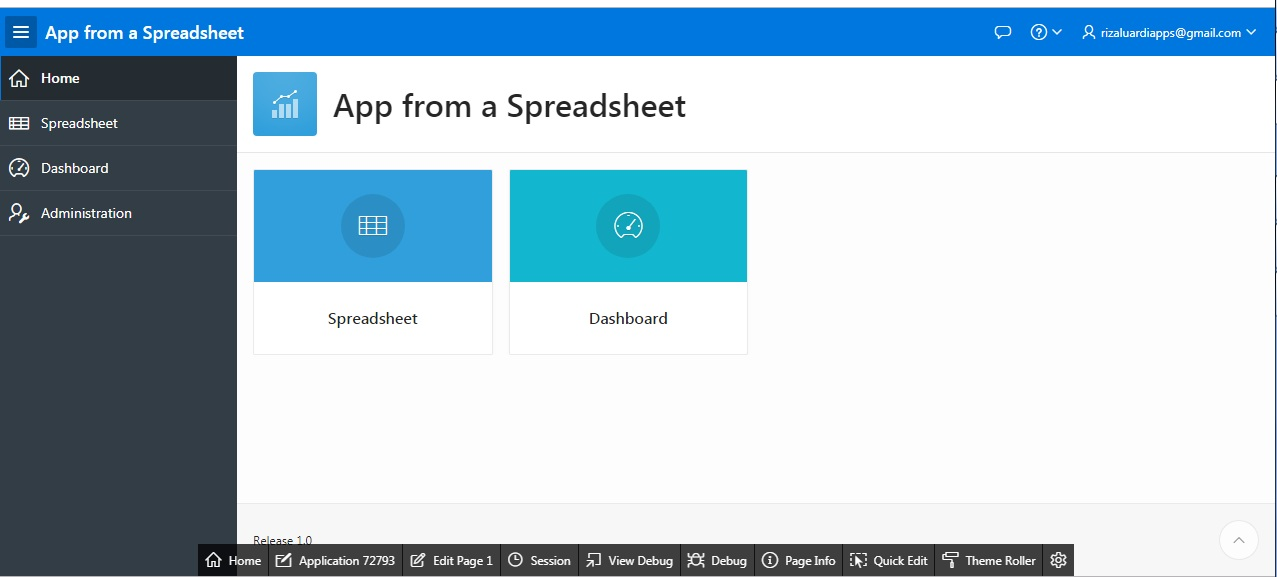
\includegraphics[scale=0.4]{figures/congratz.jpg}
    \caption{\textit{Welcome Spreadsheet.}}
        \end{center}
\label{gambar}
\end{figure}

\end{enumerate}
